\documentclass{beamer}
\usepackage[utf8]{inputenc}
\usetheme{Copenhagen}
\title{A Tool For Analysis Of Dynamic Memory Allocators}
\author{Petr Muller}
\date{29.4.2010}
\begin{document}
\begin{frame}
\titlepage
\end{frame}

\begin{frame}{Introduction}
\begin{itemize}
\item Allocator = malloc/free interface
\item Ubiquitous and essential
\item Vendor distributed performs well for usual scenarios
\item More performance can be gained by using specialized allocator
\end{itemize}
\end{frame}

\begin{frame}{Performance}
Temporal and spatial efficiency
\begin{itemize}
\item Temporal efficiency: cost of allocator operations
\item Spatial efficiency: allocator does not waste memory (overhead, fragmentation)
\item Spatial characteristics affect also temporal performance (cache interactions)
\item Efficiency depends on usage patterns (online algorithm)
\end{itemize}
\end{frame}

\begin{frame}{Tool purpose}
Analyse various metrics of an allocator under arbitrary usage pattern

\begin{itemize}
\item Usage pattern represented as "scenario files"
\item Written / captured pattern of another program
\item Translated to C
\item Executed, monitored, analysed
\end{itemize}
\end{frame}

\begin{frame}[fragile]
\frametitle{Scenario file example}
\begin{verbatim}
workjob w1 = {
  alloc one 40
  alloc two 24
  alloc three 30
  work write whole two sequential
  dealloc one
  dealloc two
  dealloc three
}

thread 1 does workjob w1 times 1000000
thread 2 does workjob w1 times 500000
thread 3 does workjob w1 times 600000

\end{verbatim}
\end{frame}

\begin{frame}{Data collection and analysis}
\begin{itemize}
\item Modular system of ``probes''
\item Only one metric is collected during one session (interference)
\item Raw data analysed after testcase execution
\item Text and visual outputs, as defined by probe
\end{itemize}
Probe types:
\begin{itemize}
  \item Total scenario time
  \item Request cost
  \item Fragmentation and overload (indistinguishable)
  \item Locality and cache friendliness
\end{itemize}
\end{frame}

\begin{frame}[fragile]
\frametitle{Example 1: Simple total time}
\tiny
\begin{verbatim}
$ ./benchmark.py probe --allocator=/lib64/libc-2.11.1.so --probe=totaltime\
                       --scenario=scenarios/small-lot.alloc -b=3 -c=5
Loading the probe                                  [ PASS ]
Probe validation                                   [ PASS ]
Probe preparation                                  [ PASS ]
================================================================================
Statistics:  User time
Mean:                26.662000
Standard deviation:  0.010954
Standard error:      0.004382
Min         Q1         Median     Q3         Max       
---         --         ------     --         ---
26.650000   26.650000  26.670000  26.670000  26.670000

Statistics:  Real time
Mean:                15.128000
Standard deviation:  0.078230
Standard error:      0.031292
Min         Q1         Median    Q3          Max       
---         --         ------    --          ---
15.020000   15.080000  15.160000 15.160000   15.220000

(...omitted...)
================================================================================
Probe run                                          [ PASS ]
\end{verbatim}

\end{frame}

\begin{frame}{Example 2: memory usage graph}
    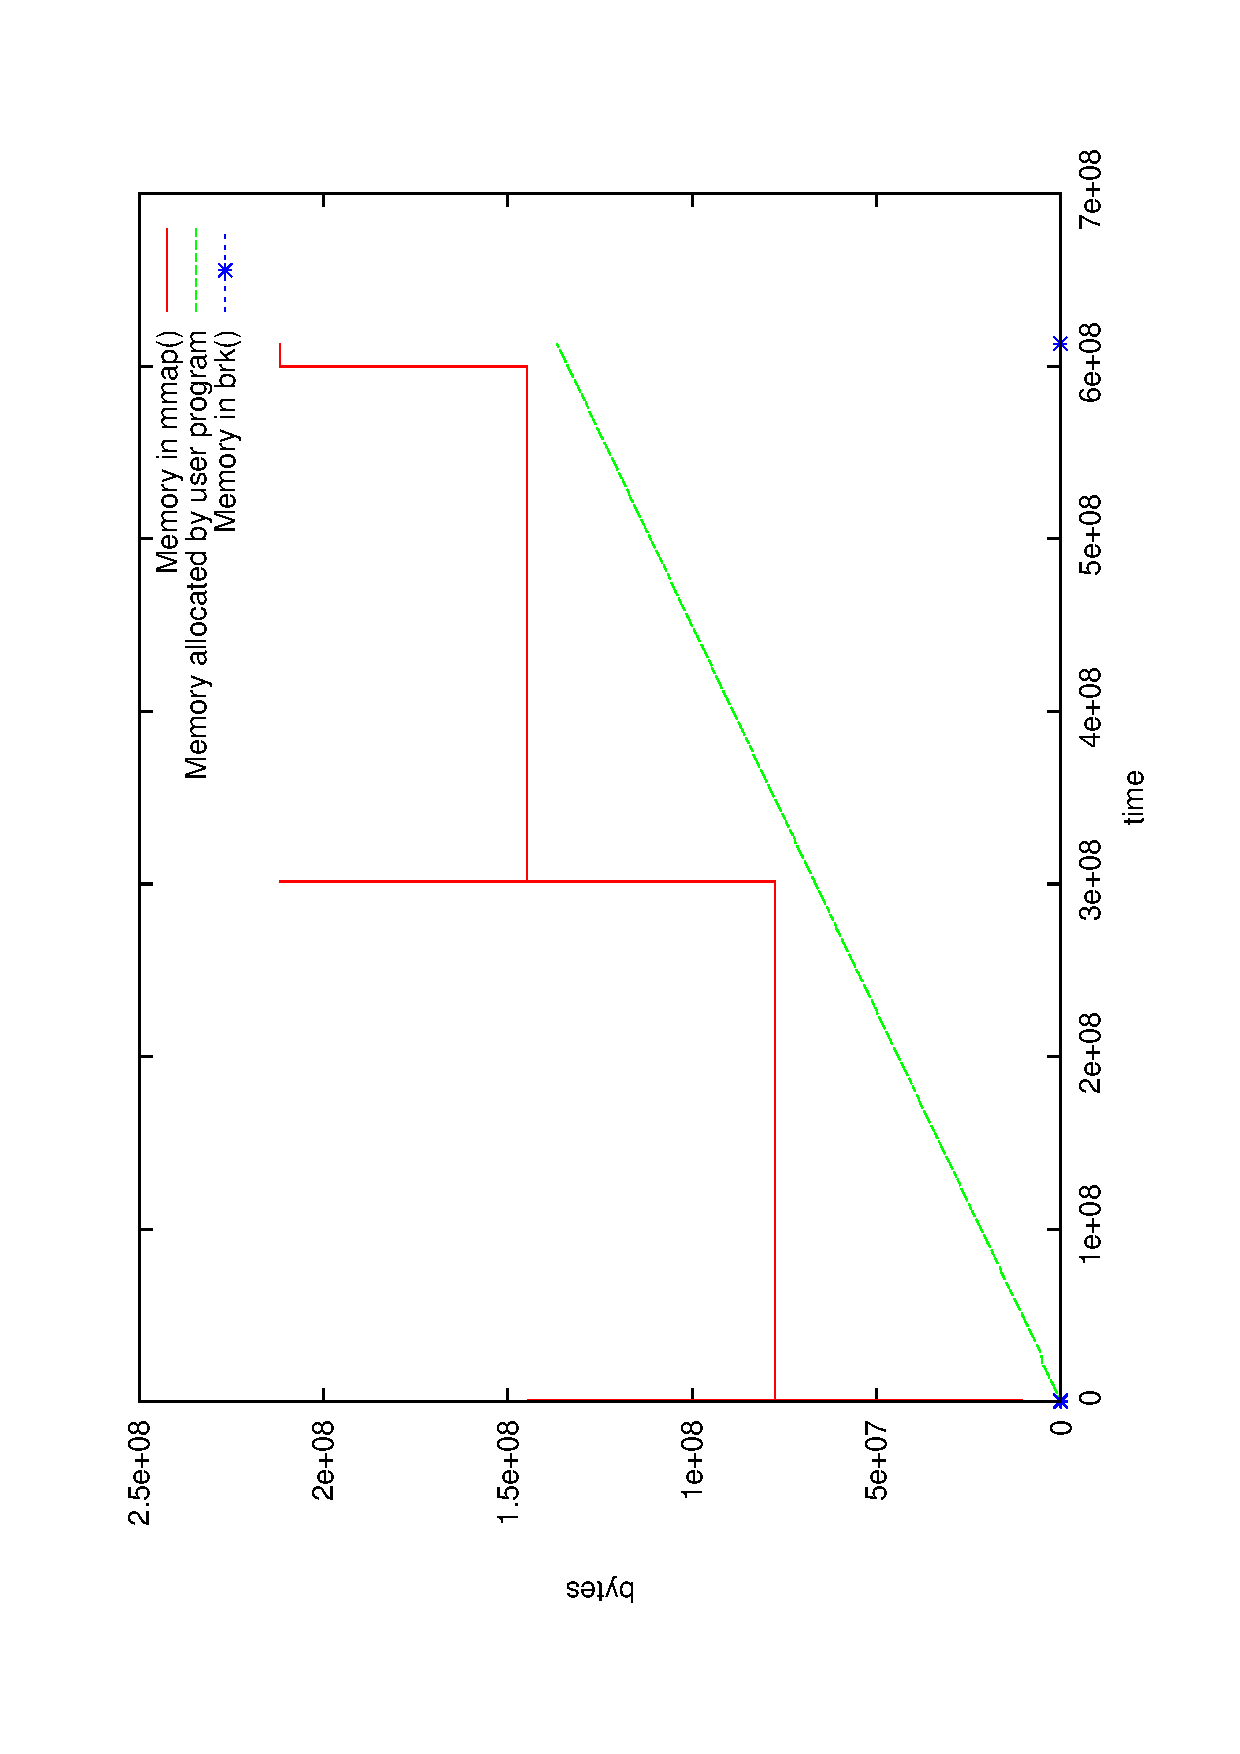
\includegraphics[scale=0.4]{memory}
\end{frame}

\end{document}
